\subsection*{Aufgabe 2}

\subsubsection*{a)}

Es soll das elektrostatsische Potential auf der x-Achse gemäß
\begin{equation}
  \Phi(x) = \frac{1}{4 \pi \varepsilon_0} \int \int \int \frac{\rho(x', y', z')}{((x-x')^2+y'^2+z'^2)^{\sfrac{1}{2}}} \mathrm{d}x'\mathrm{d}y'\mathrm{d}z'
  \label{eqn:phi}
\end{equation}
mit einer homogenen Ladungsverteilung
\begin{equation*}
  \rho(x, y, z) = \begin{cases}
  \rho_0 & |x|,|y|,|z| < a \\
  0 &\, \text{sonst}
\end{cases}
\end{equation*}
berechnet werden.

Das gegebene Integral wird dafür zunächst einheitenlos gemacht. Dafür werden folgende Ersetzungen vorgenommen:
\begin{align*}
    \tilde{x} &= \frac{x}{a} \\
    \tilde{\Phi} &= \frac{4 \pi \varepsilon_0}{\rho_0 a^2} \Phi.
\end{align*}
Zusätzlich wird \(a = 1\) gesetzt. Damit ergibt sich
\begin{equation*}
  \tilde{\Phi}(x) = \int_{-1}^1 \int_{-1}^1 \int_{-1}^1 \frac{1}{((x-x')^2+y'^2+z'^2)^{\sfrac{1}{2}}} \mathrm{d}x'\mathrm{d}y'\mathrm{d}z'.
\end{equation*}

Das Potential außerhalb des Würfels kann mithilfe einer Multipolentwicklung zur ersten nicht verschwindenden Ordnung, also dem Monopol-Moment, genähert werden
\begin{equation*}
  \tilde{\Phi}(x) \: \propto \: \frac{1}{\rho_0 |x|} \int \int \int \rho(x', y', z') \mathrm{d}x'\mathrm{d}y'\mathrm{d}z' = \frac{1}{|x|}.
\end{equation*}
In Abbildung \ref{fig:aus_a} sind \(\tilde{\Phi}(x)\) sowie die Näherung aufgetragen. Daran ist zu sehen, dass die Näherung den Trend der Werte sehr gut abbildet.
In Abbildung \ref{fig:inn_a} ist das Potential innerhalb des Würfels aufgetragen.
Beim Integrieren könnte der Nenner Null werden, wodurch das Integral divergiert. Um dies zu verhindern, kann ein kleines \(\varepsilon\) auf denn Nenner addiert werden, sobald dieser zu klein wird. Alternativ kann auch eine andere Anzahl an Teilintervallen \(n\) gewählt werden.
\begin{figure}
  \centering
  \begin{subfigure}[b]{0.45\textwidth}
      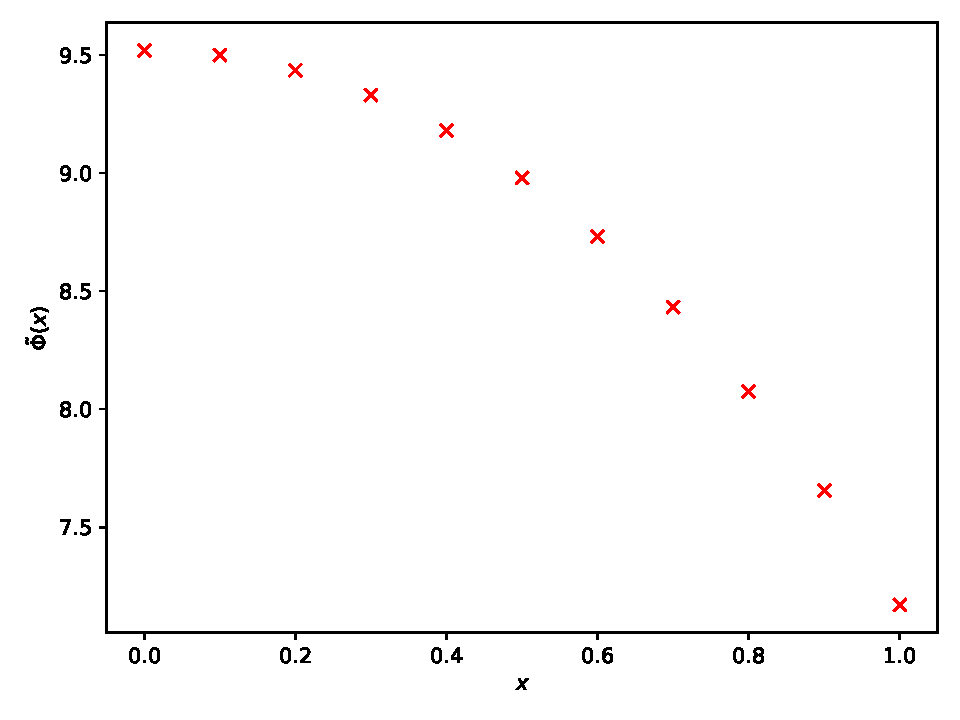
\includegraphics[width=\textwidth]{A2/build/innerhalb_a.pdf}
      \caption{Potential innerhalb des Würfels.}
      \label{fig:inn_a}
    \end{subfigure}
    ~ %add desired spacing between images, e. g. ~, \quad, \qquad, \hfill etc.
    %(or a blank line to force the subfigure onto a new line)
    \begin{subfigure}[b]{0.45\textwidth}
      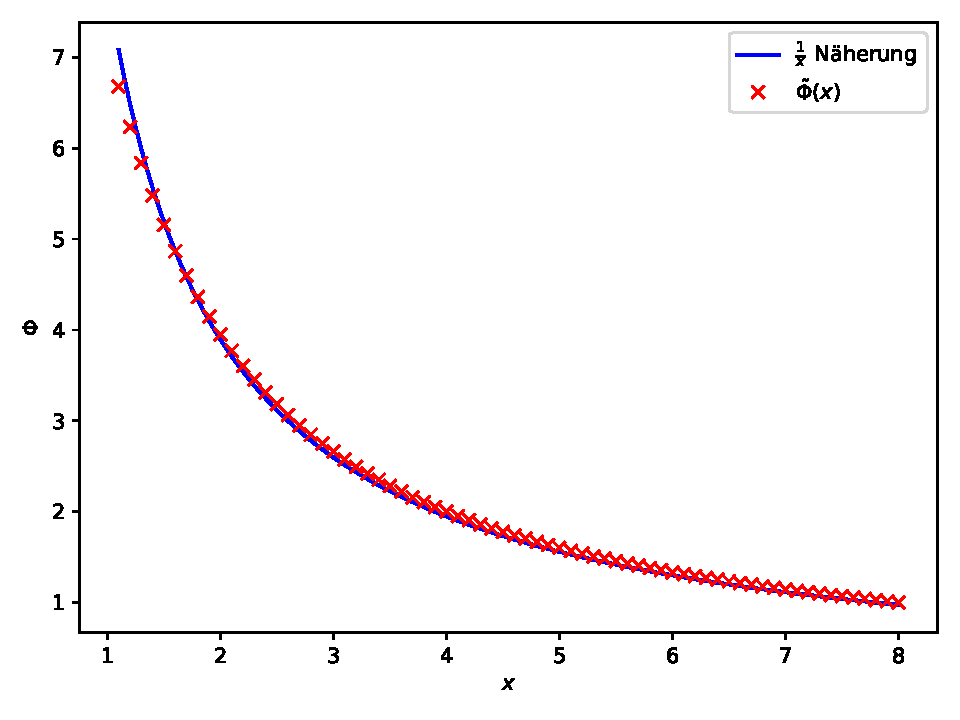
\includegraphics[width=\textwidth]{A2/build/ausserhalb_a.pdf}
      \caption{Potential außerhalb des Würfels.}
      \label{fig:aus_a}
    \end{subfigure}
    \caption{Berechnung von \(\tilde{\Phi}(x)\).}\label{fig:a}
\end{figure}

\subsubsection*{b)}

Nun soll das elektrostatsische Potential \eqref{eqn:phi} mit der Ladungsverteilung
\begin{equation*}
  \rho(x, y, z) = \begin{cases}
  \rho_0 \frac{x}{a} & |x|,|y|,|z| < a \\
  0 &\, \text{sonst}
  \end{cases}
\end{equation*}
bestimmt werden. Da \(x\) und \(a\) die gleiche Einheit besitzen, können dieselben Ersetzungen wie in a) verwendet werden, um das Integral einheitenlos zu machen. Auch hier wird \(a=1\) gesetzt.
Damit ergibt sich
\begin{equation*}
  \tilde{\Phi}(x) = \int_{-1}^1 \int_{-1}^1 \int_{-1}^1 \frac{x}{((x-x')^2+y'^2+z'^2)^{\sfrac{1}{2}}} \mathrm{d}x'\mathrm{d}y'\mathrm{d}z'.
\end{equation*}
Die erste nicht verschwindende Ordnung der Multipolentwicklung stellt dieses Mal das Dipol-Moment dar. Das Potential außerhalb des Würfels kann damit als
\begin{equation*}
  \tilde{\Phi}(x) \: \propto \: \frac{\vec{e}_\text{r}}{\rho_0 x^2} \int \int \int \vec{r}' \rho(x', y', z') \mathrm{d}x'\mathrm{d}y'\mathrm{d}z' = \frac{1}{x^2}
\end{equation*}
genähert werden.
In Abbildung \ref{fig:aus_b} ist \(\tilde{\Phi}(x)\) und in Abbildung \ref{fig:aus_b_fit} die Näherung aufgetragen. Dieses Mal beschreibt die Näherung die tatsächlichen Werte nur sehr schlecht, was möglicherweise daran liegt, dass die Terme höherer Ordnung in diesem Fall einen großen Einfluss auf den Verlauf von \(\tilde{\Phi}(x)\) haben.
\begin{figure}
  \centering
  \begin{subfigure}[b]{0.45\textwidth}
      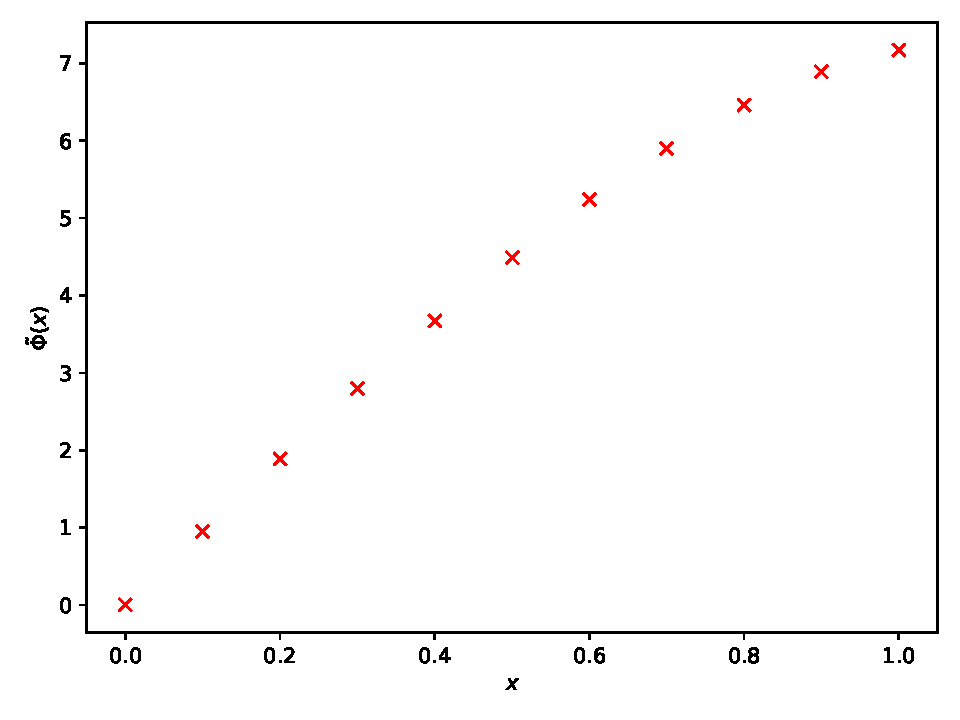
\includegraphics[width=\textwidth]{A2/build/innerhalb_b.pdf}
      \caption{Potential innerhalb des Würfels.}
      \label{fig:inn_b}
    \end{subfigure}
    ~ %add desired spacing between images, e. g. ~, \quad, \qquad, \hfill etc.
    %(or a blank line to force the subfigure onto a new line)
    \begin{subfigure}[b]{0.45\textwidth}
      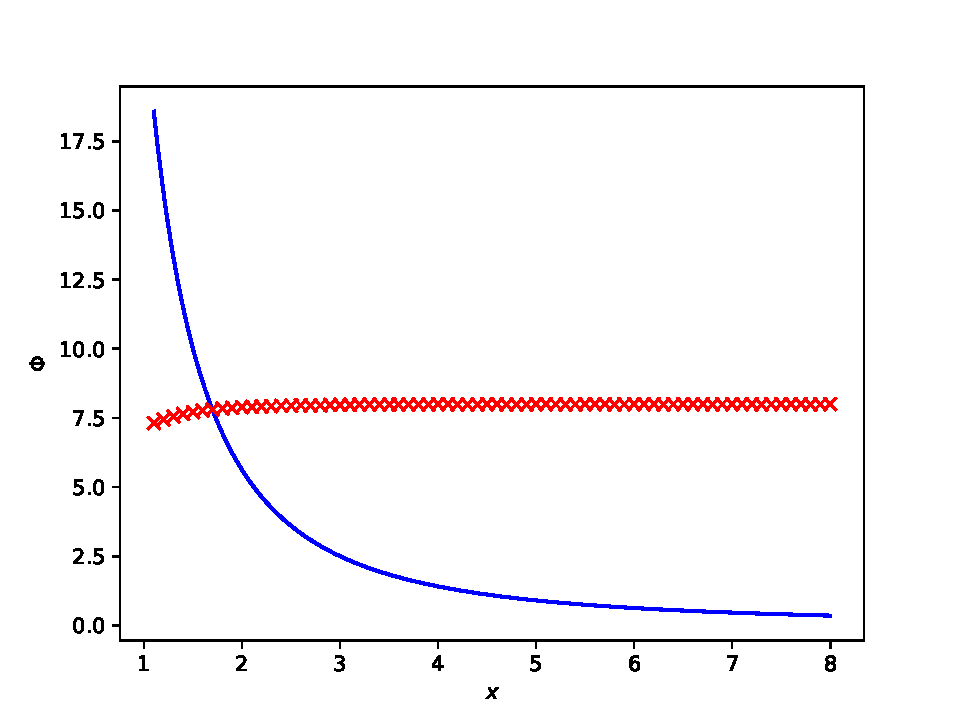
\includegraphics[width=\textwidth]{A2/build/ausserhalb_b.pdf}
      \caption{Potential außerhalb des Würfels.}
      \label{fig:aus_b}
    \end{subfigure}
    ~
    \begin{subfigure}[b]{0.45\textwidth}
      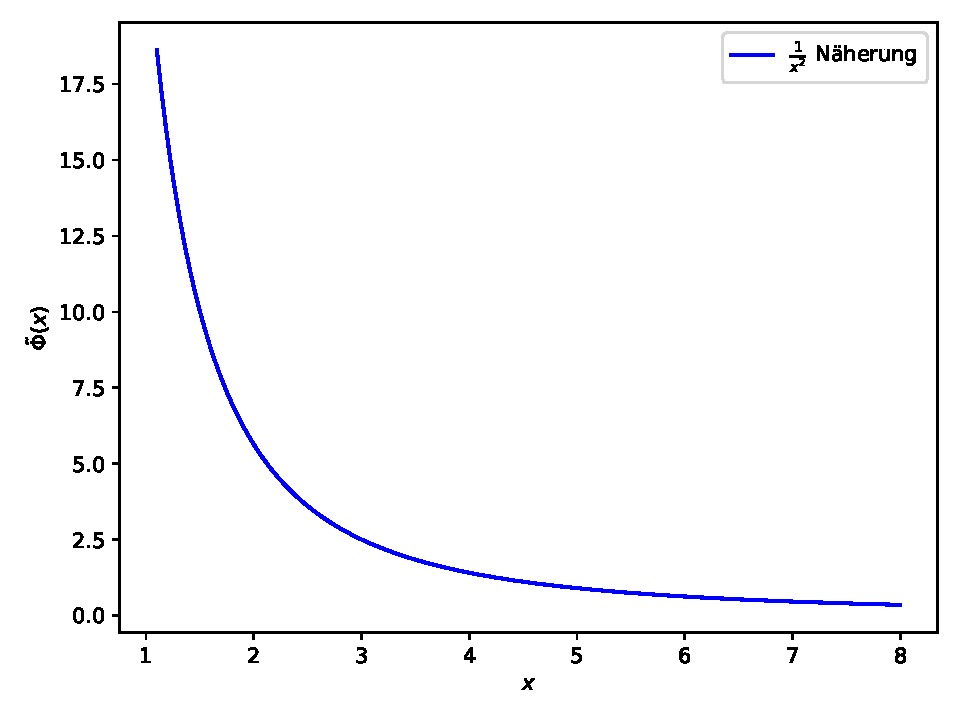
\includegraphics[width=\textwidth]{A2/build/ausserhalb_b_fit.pdf}
      \caption{Näherung des Potential außerhalb des Würfels.}
      \label{fig:aus_b_fit}
    \end{subfigure}
    \caption{Berechnung von \(\tilde{\Phi}(x)\).}\label{fig:b}
\end{figure}
